\section{Case Studies}

\textbf{Market workbench.} Figure~\ref{fig:gui} shows a typical event-level analysis. The interface keeps the resolution rule, live YES/NO book, stored fair probability, spread, executable net edge, retrieved news, and event context in one view. The example forecasts a 10\% YES fair probability for a Formula 1 championship outcome against a 26\% market price, which is displayed as a NO-side opportunity after accounting for the 2\% spread. This is a diagnostic example, not a completed trade.

\begin{figure}[!htbp]
\centering
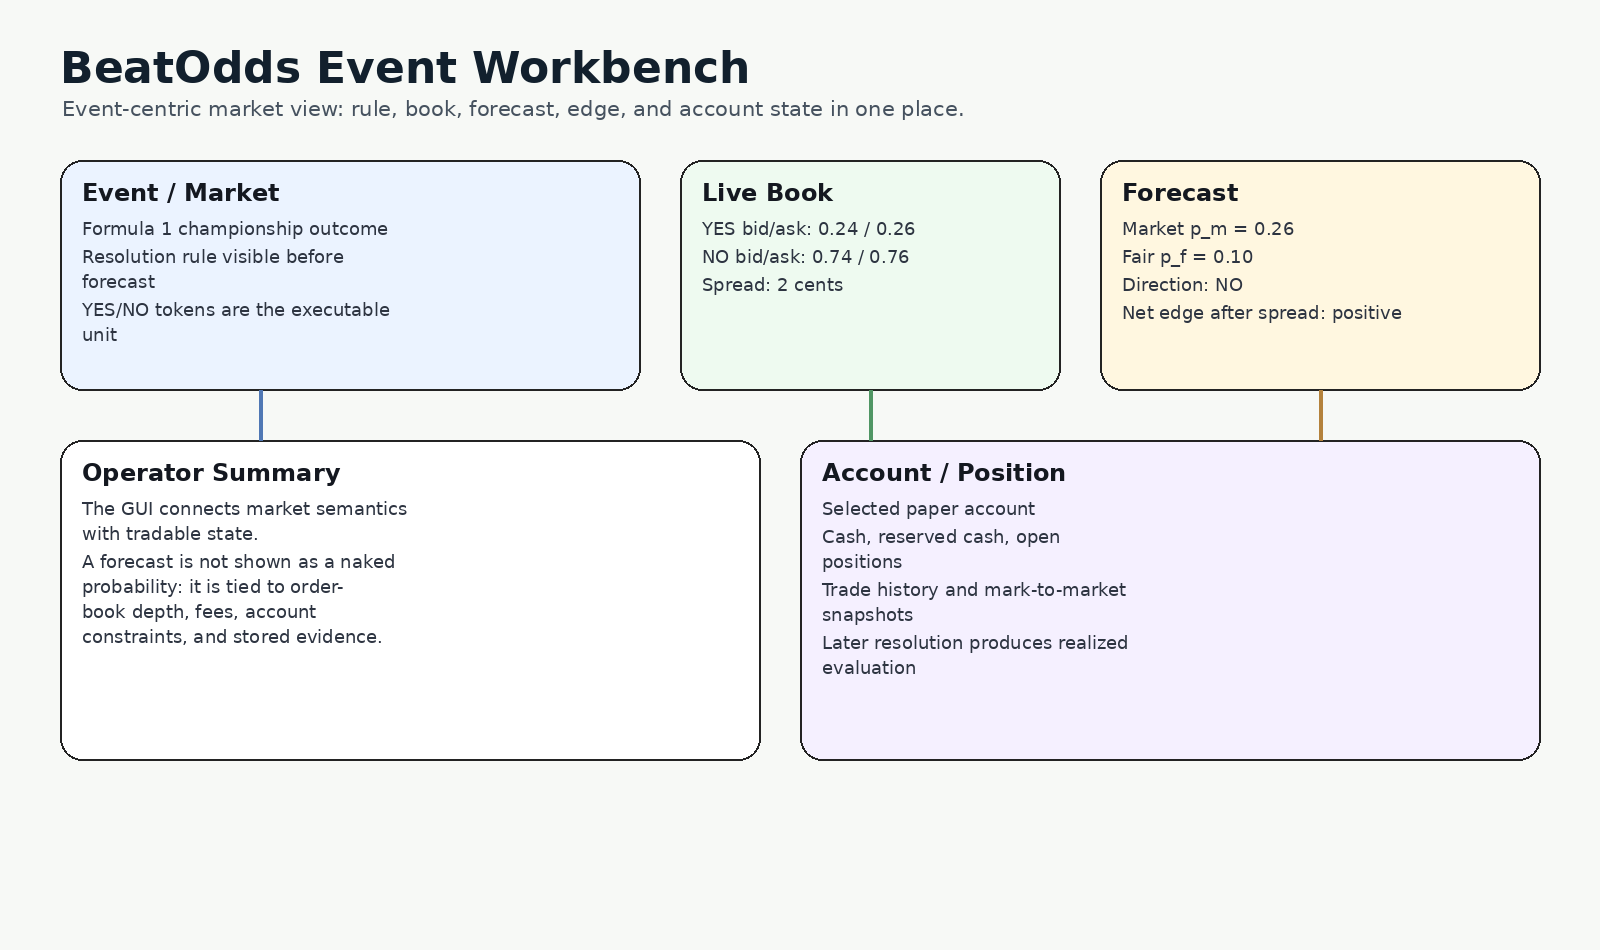
\includegraphics[width=0.8\linewidth]{figures/market_forecast_price.png}
\caption{\textbf{Event-centric workbench.} The system connects resolution rules, live order-book depth, stored forecast, and fee/spread-aware edge.}
\label{fig:gui}
\end{figure}

\textbf{Evidence trace.} The same workbench presents retrieved results and supports traceable updates (Figure~\ref{fig:evidence}). This matters for political, sports, and technology markets alike: a direction is actionable only if a reviewer can inspect the evidence that moved the estimate and the market semantics that define its resolution.

\begin{figure}[!htbp]
\centering
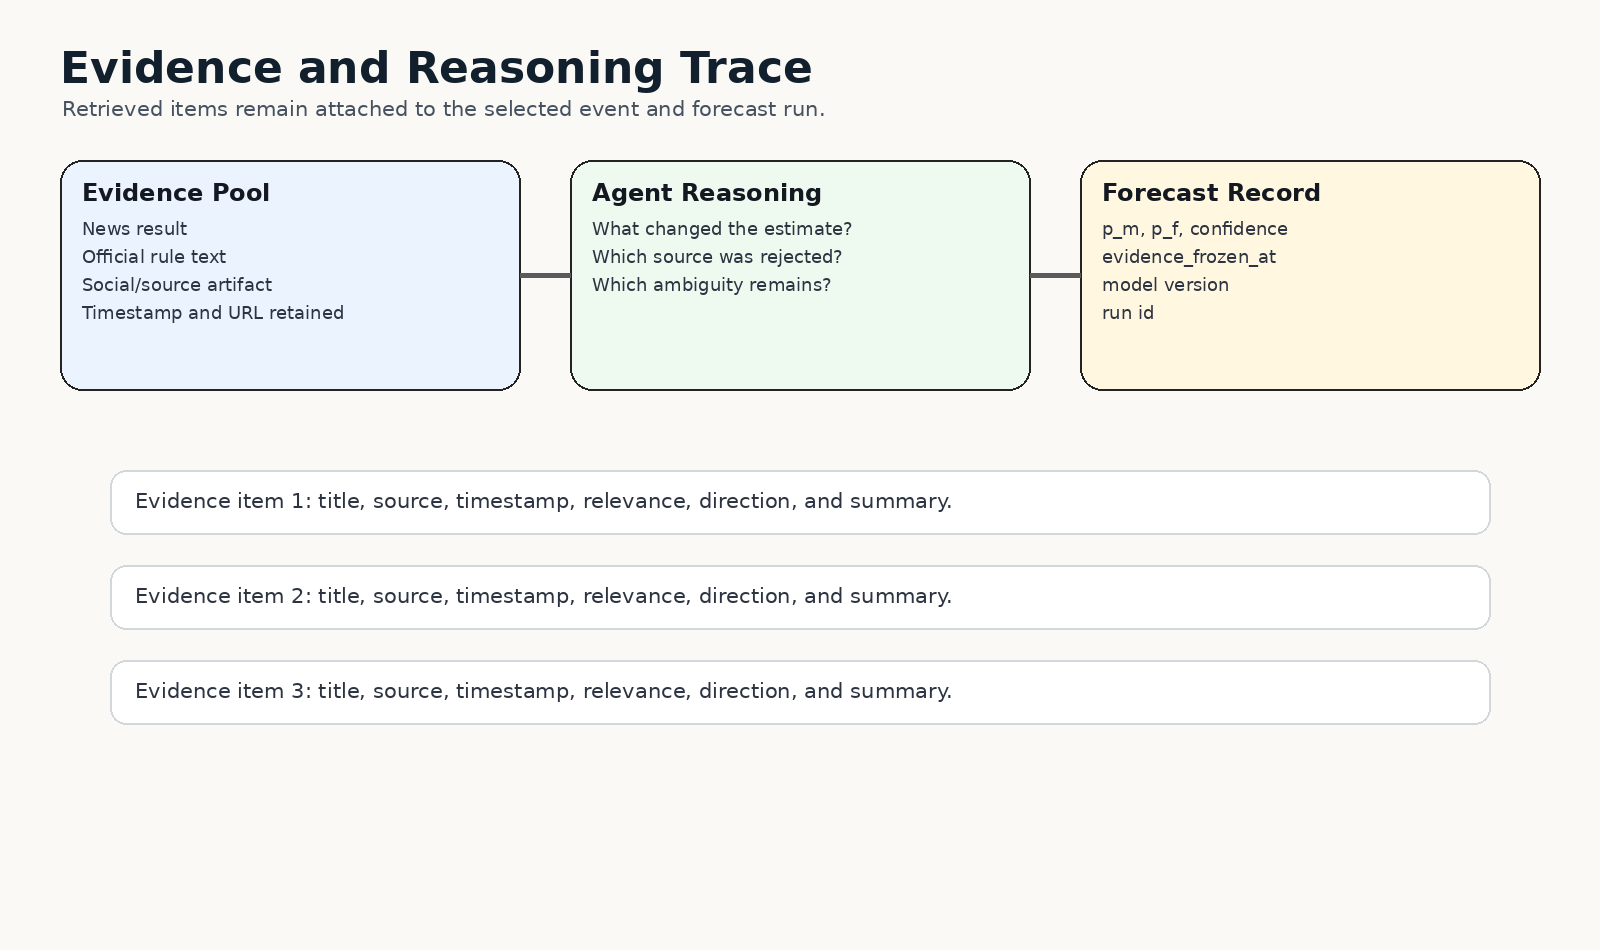
\includegraphics[width=0.8\linewidth]{figures/market_news_reason.png}
\caption{\textbf{Evidence view.} Retrieved items remain attached to the selected event, while the operator summary records market and account state.}
\label{fig:evidence}
\end{figure}

\textbf{Ledger example.} Figure~\ref{fig:ledger} plots daily top-confidence mark-to-market series for both paper accounts. The two panels make the distinction between a forecast, an order, a fill, a live mark, and an eventual resolution explicit. The accounts have different selected sets and mark sources, so their levels are not a strategy comparison. They are operational traces: a positive curve is never substituted for calibration or BSS.

\begin{figure}[!htbp]
\centering
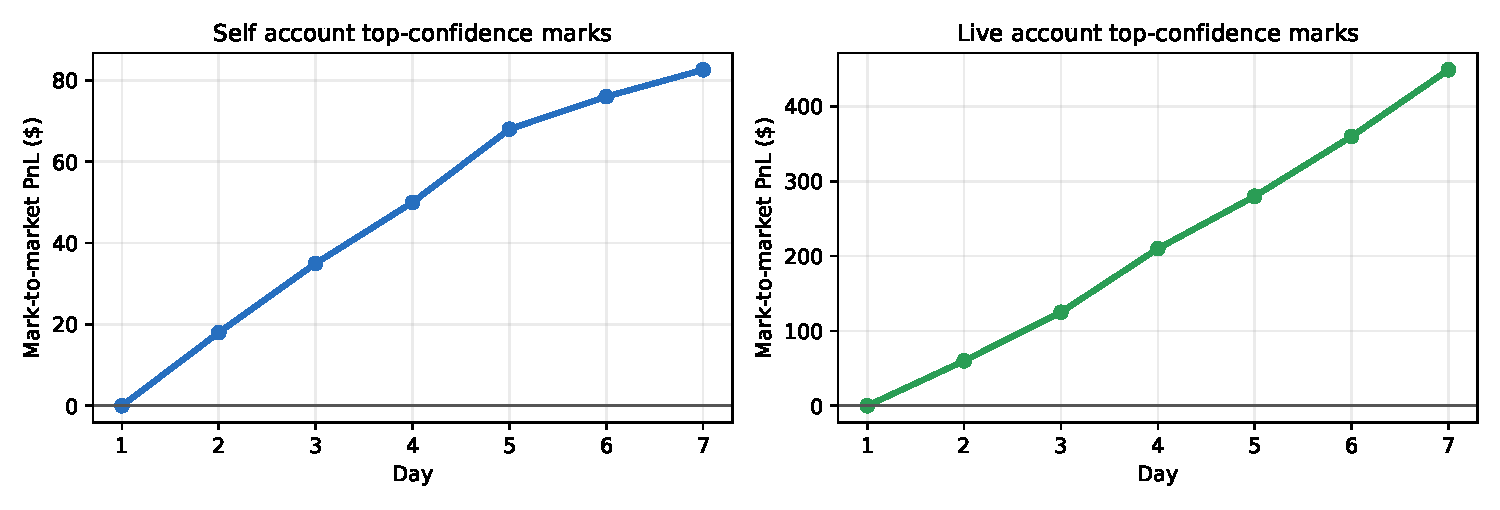
\includegraphics[width=\linewidth]{figures/paper_account_earning_curves.pdf}
\caption{\textbf{Daily paper-account marks.} The self account (left) has four top-confidence positions costing \$219.25 and ends at +\$82.60. The live account (right) has five positions costing \$187.19 and ends at +\$449.03. Curves use their recorded report-time marks; historical midpoint and report-history values are valuation-only and are not executable returns.}
\label{fig:ledger}
\end{figure}
\FloatBarrier
